\chapter{基于多模态大语言模型的GBM候选分子生成框架}\label{chap:framework}

\section{引言}\label{sec:ch3-intro}

本章系统阐述GBM-PharmaMind候选分子生成框架的设计理念与具体实现。3.2节说明系统总体架构与设计思路；3.3节至3.6节分别介绍GBM多模态知识库、Prompt生成器、分子图—文本协同生成模块和GBM领域LoRA适配；3.7节给出CoT-ToT协同生成算法；3.8节与3.9节进一步说明物理评估反馈机制和最终候选分子排序机制。

\section{系统总体架构与设计思路}\label{sec:system-arch}

本文提出了GBM-PharmaMind框架，以具备分子图—文本协同生成能力的多模态大模型Llamole为基础[24]，实现了涵盖知识引导、多模态生成、物理验证和反馈调整的端到端流水线。系统架构如图3.1所示。

\begin{figure}[htbp]
    \centering
    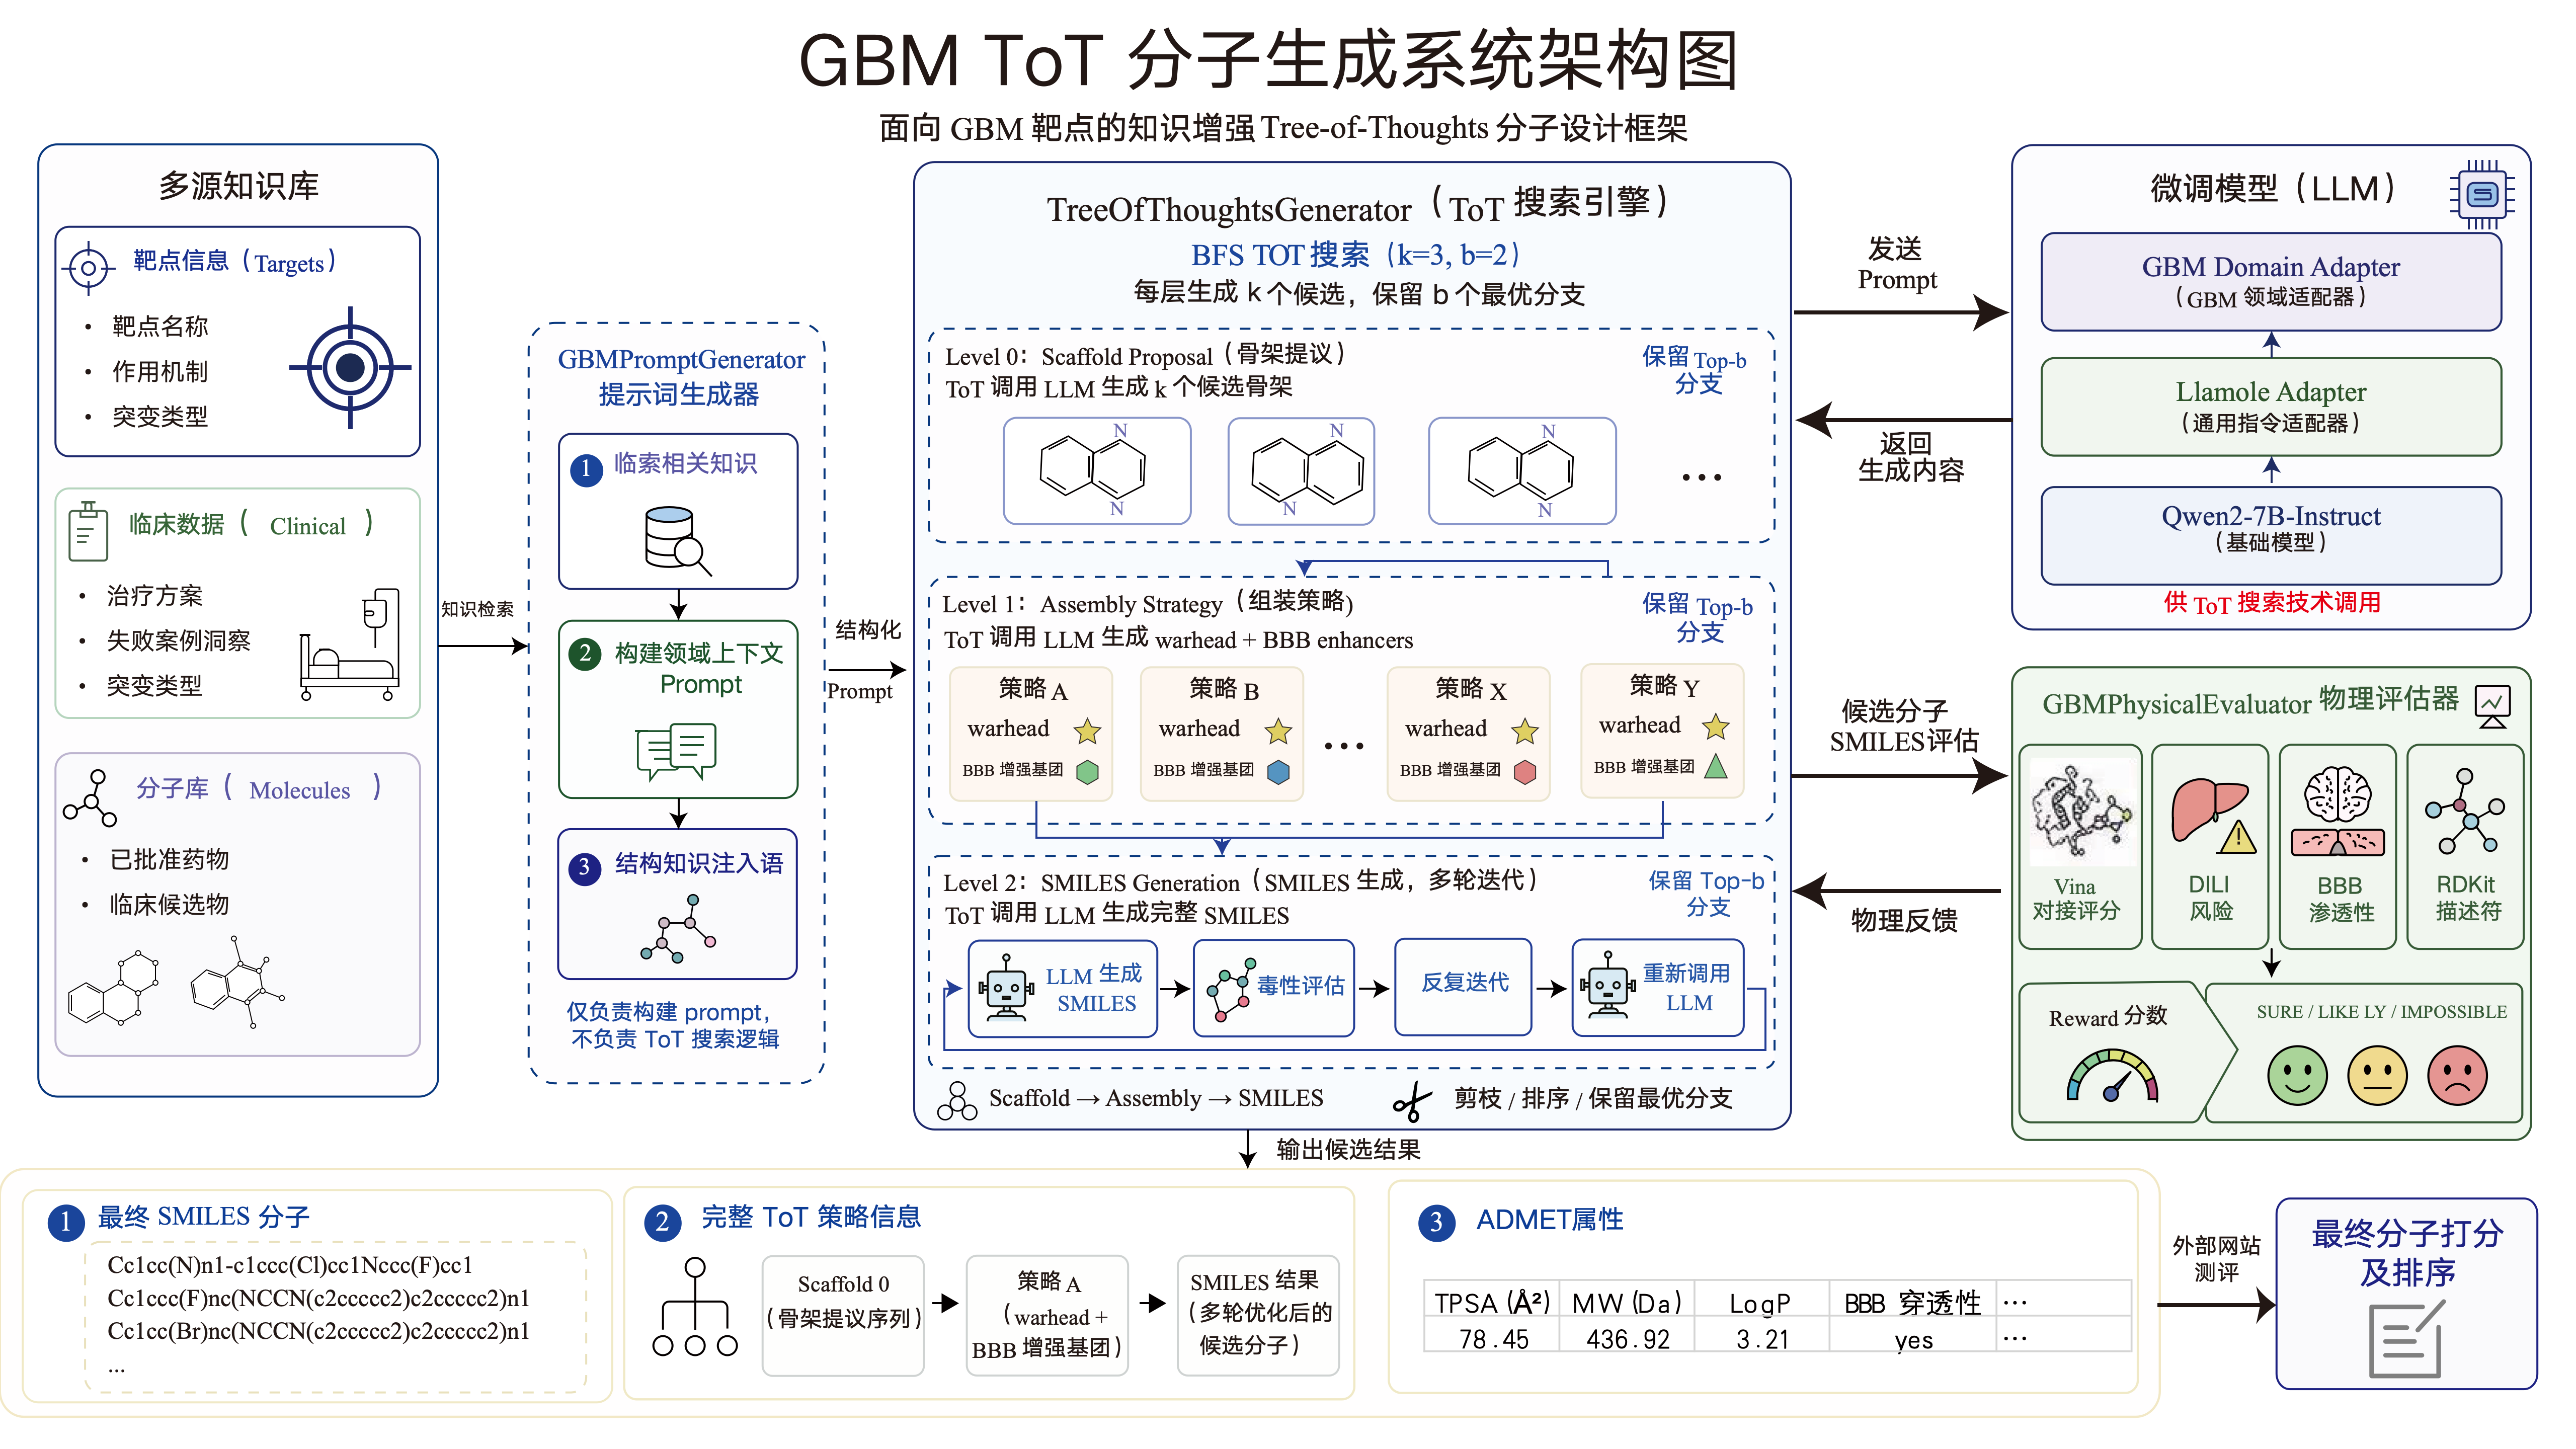
\includegraphics[width=0.9\textwidth]{图片/系统架构图.png}
    \caption{GBM候选分子生成系统架构图}\label{fig:system-arch}
\end{figure}

GBM候选分子生成涉及疾病靶点背景、CNS成药性约束和后续计算评价等多类信息，如果这些信息只在生成结束后统一筛选，容易造成大量候选结构在后续评估阶段被剔除。因此，本文在框架设计中将知识输入、结构生成和物理反馈三个环节前置到同一生成流程中，使候选分子在生成阶段就受到GBM任务条件的约束。

在输入端，系统接收目标靶点名称、生成分子数量上限以及配置需求。GBM领域知识库根据靶点名称返回相关靶点背景、CNS药物设计规则、参考分子结构和风险提示，Prompt生成器再将这些信息组织为模型可读取的任务输入。在生成端，Llamole负责完成文本条件到分子图结构的映射，CoT-ToT策略则进一步将候选分子设计过程拆分为骨架提议、片段组装和SMILES生成三个阶段。生成得到的候选结构随后进入物理评估模块，接受SMILES解析、理化性质检查、BBB经验评分、Vina对接和结构风险检测，这一模块的评价结果用于生成阶段的剪枝和反馈。

系统输出包括两个层次。第一层次是生成阶段输出，主要包括候选分子SMILES、分阶段推理结果以及对应的中间评价信息。第二层次是排序阶段输出，即经过外部工具重新计算和综合评分后的Top候选分子列表。通过这种设计，GBM-PharmaMind能够将疾病知识、多模态生成和计算评价组织为连续流程。

\section{GBM多模态知识库构建}\label{sec:knowledge-base}

\subsection{GBM领域知识库的构建必要性}

GBM候选分子生成对领域知识具有较强依赖。与一般分子生成任务相比，GBM任务不仅需要关注靶点结合潜力，还需要同时考虑BBB限制、CNS药物理化要求以及既有治疗经验。若仅向模型提供靶点名称，生成过程容易退化为通用化学空间中的结构采样，难以体现GBM任务的疾病特异性。因此，本文构建GBM多模态知识库，为后续Prompt生成、LoRA适配和物理评估提供统一的领域输入。该模块要求：知识库中的内容不仅用于背景说明，还需要能够转化为Prompt约束、LoRA适配数据和候选分子评价参考。

\subsection{ GBM 领域知识库构建与生成约束注入}

本文将知识库划分为GBM靶点信息库、GBM临床治疗数据库、GBM分子参考数据库和结构知识库四个部分。四类知识并不是相互独立的背景材料，而是在Prompt构建过程中共同提供靶点背景、临床约束、参考结构和分子设计规则。通过这种组织方式，模型在生成候选分子时不仅能够获得靶点名称，还能够同时接收与GBM疾病背景、CNS成药性要求和结构风险相关的约束信息。

GBM靶点信息库主要记录候选分子生成所需的疾病靶点背景。本文重点整理EGFR、VEGF/VEGFR和IDH1/IDH2等代表性靶点的信息。其中，EGFR是GBM中研究较成熟且突变频率较高的靶点，已有较多抑制剂结构和母核信息可作为生成参考\cite{Fu2025}；VEGF/VEGFR与肿瘤血管生成密切相关，但抗血管生成治疗在总体生存改善方面仍存在局限，因此相关候选分子生成需要考虑该靶点作用机制的复杂性\cite{Fu2025}；IDH1/IDH2与代谢重编程和分子分型相关，突变体口袋结构相对明确，适合用于对接评估和候选分子筛选\cite{Fu2025}。围绕这些靶点，知识库中记录靶点名称、相关分子亚型、突变或表达特征、已知抑制剂或药物、推荐分子量范围、推荐LogP范围、BBB相关要求以及设计风险提示等字段。

GBM临床治疗数据库用于补充疾病治疗背景和临床经验。标准治疗方案和TMZ耐药机制是理解GBM治疗现状的重要基础\cite{Stupp2005}，而BBB限制则是CNS药物设计中必须前置考虑的核心约束\cite{Pardridge2012}。这些信息进入Prompt后，可以帮助模型避免仅围绕靶点结合活性生成分子，而忽略脑部递送和治疗背景。与此同时，部分失败临床试验所反映的问题也可作为风险提示，用于减少重复已知低效策略的可能性\cite{Fu2025}。

GBM分子参考数据库主要保存已获批药物、临床试验分子以及相关候选结构的信息。本文将替莫唑胺等已知CNS药物结构作为参考，使模型能够学习已有药物的结构特点\cite{Stupp2005}；同时，临床试验分子的骨架类型和设计原则也被纳入数据库，为后续骨架提议和片段组装提供结构参照\cite{Fu2025}。结构知识库则进一步补充药物化学层面的规则信息，包括BBB优化基团、PAINS警告结构和Lipinski五规则等内容。BBB优化基团如烷氧基取代和氮杂环可为提高BBB穿透倾向提供设计参考\cite{Ferraris2020}；PAINS警告结构需要在生成阶段进行规避，以减少泛筛选干扰化合物的产生\cite{Baell2010}；Lipinski五规则则作为类药性判断的基础依据\cite{Pardridge2012}。

实际调用过程中，知识库先根据目标靶点名称检索对应的靶点背景和设计字段，再补充临床治疗经验、参考分子结构以及结构风险提示。系统通过结构化模板将上述信息写入Prompt，使靶点背景、BBB约束、结构风险和参考骨架能够在生成阶段共同参与分子设计。

该过程如算法\ref{alg:kb-prompt}所示。

\begin{algorithm}
\caption{基于知识库检索的Prompt构建算法}
\label{alg:kb-prompt}
\textbf{输入}：目标靶点名称$T$、知识库$K$、理化约束$C$ \\
\textbf{输出}：携带GBM领域知识的完整Prompt $P_T$

\begin{algorithmic}[1]
\Function{BuildKnowledgePrompt}{$T, K, C$}
    \State $\text{target\_info} \leftarrow \text{KB.get\_target\_info}(T)$    \Comment{从靶点信息库检索靶点背景}
    \State $\text{clinical\_insights} \leftarrow \text{KB.get\_clinical\_insights}()$    \Comment{从临床数据库检索治疗洞察}
    \State $\text{reference\_mols} \leftarrow \text{KB.get\_similar\_molecules}(T, \text{limit}=3)$    \Comment{从分子库检索参考骨架}
    \State $\text{structural\_guidance} \leftarrow \text{StructuralInjector.inject}(T)$    \Comment{从结构知识库注入骨架与BBB指导}
    \State $\text{bbb\_constraint} \leftarrow \text{FormatBBB}(\text{target\_info})$    \Comment{读取BBB约束字段（MW上限、TPSA上限）}
    \State $\text{risk\_warning} \leftarrow \text{FormatRisk}(\text{target\_info})$    \Comment{读取结构风险提示（如EGFRvIII变体风险）}
    \State $\text{template} \leftarrow \text{LoadPromptTemplate}(T)$    \Comment{加载靶点对应的Prompt模板}

    \State $P_T \leftarrow \text{template.format}($
        \Statex \hspace{1.2em} $\text{靶点背景}=\text{target\_info.description},$
        \Statex \hspace{1.2em} $\text{临床洞察}=\text{clinical\_insights},$
        \Statex \hspace{1.2em} $\text{参考骨架}=\text{reference\_mols},$
        \Statex \hspace{1.2em} $\text{结构指导}=\text{structural\_guidance},$
        \Statex \hspace{1.2em} $\text{BBB约束}=\text{bbb\_constraint},$
        \Statex \hspace{1.2em} $\text{风险提示}=\text{risk\_warning},$
        \Statex \hspace{1.2em} $\text{理化约束}=C$
    \State $)$
    \State \Return $P_T$
\EndFunction
\end{algorithmic}
\end{algorithm}

算法\ref{alg:kb-prompt}展示了知识库到Prompt的转换过程。目标靶点输入后，系统依次读取靶点信息、临床洞察、参考骨架和结构指导，并将BBB约束、风险提示和理化约束写入统一模板。通过该流程，分散的GBM领域知识被整理为生成模型可直接读取的结构化输入，从而为后续LoRA适配、CoT-ToT生成和物理评估反馈提供基础。

\section{Prompt生成器设计}\label{sec:prompt-generator}

\subsection{Prompt生成器的设计必要性}

LLM的输出质量高度依赖输入Prompt的设计~\cite{Wei2022,jin2025effective}。在分子生成任务中，Prompt需要包含以下要素：

\begin{itemize}
    \item \textbf{靶点背景}用于帮助LLM理解"EGFR"等靶点名称所对应的生物学含义~\cite{Fu2025}；
    \item \textbf{显式理化约束}用于增强模型对MW、LogP、TPSA等数值条件的遵循能力~\cite{Pardridge2012}；
    \item \textbf{风险结构约束}用于在生成阶段减少PAINS、DILI和hERG等潜在风险结构的出现~\cite{Aronov2008}；
    \item \textbf{CoT步骤}用于将复杂的分子设计任务拆分为可检查的中间过程~\cite{Wei2022}。
\end{itemize}

设目标靶点为$T$，知识库中与该靶点相关的领域信息为$K_T$，生成约束集合为$C$，推理格式约束为$H$，则Prompt生成器可表示为：
$$P_T = G(T, K_T, C, H)$$
其中，$G(\cdot)$表示Prompt生成函数。生成后的$P_T$同时包含靶点背景，理化性质范围、结构风险提示和输出格式要求，用于使不同靶点在统一约束体系下进入生成流程。

\subsection{Prompt生成器的核心方法}

具体而言，\texttt{generate\_full\_prompt()}负责构建完整任务输入；\texttt{build\_tot\_propose\_prompt()}负责生成骨架提议、片段组装和SMILES输出三个阶段的ToT提示；\texttt{build\_feedback\_injected\_prompt()}则用于将上一轮物理评估结果写入后续Prompt，使后续生成过程能够接收来自外部评估模块的反馈信息。

\section{分子图—文本协同生成模块}\label{sec:llamole-arch}

在GBM-PharmaMind中，Llamole承担从文本条件到分子结构的跨模态映射任务。设输入Prompt为$P_T$，语言模型首先得到隐层语义表示$h_T$，随后通过语义查询Token将该表示映射到图生成条件空间：
$$z_T = \phi(h_T)$$
其中，$\phi(\cdot)$表示图-LM连接器。图扩散模块在条件$z_T$的引导下生成候选分子图，并进一步转换为SMILES字符串。通过该过程，GBM靶点描述、BBB约束和结构风险提示能够以文本条件的形式参与分子图生成。本文不改变Llamole主体结构，而是在输入侧引入GBM知识约束，在适配侧加入LoRA，在输出侧连接物理评估反馈。

Llamole适合作为本文底层生成模型，主要原因在于其同时包含语言理解和分子图生成两部分能力。基础语言模型采用Qwen2-7B-Instruct\cite{Qwen2Team2024}，负责理解结构化分子设计任务中的靶点描述、约束条件和生成要求。为了使语言模型能够识别分子设计任务的边界，Llamole引入了特殊触发Token机制\cite{liu2025multimodal}。其中，\texttt{<design\_start>}和\texttt{<design\_end>}用于标记分子设计会话的起止，\texttt{<design\_body>}用于标记分子设计的具体内容，\texttt{<molecule>}用于标记分子结构输出位置。这些Token使模型能够在一般文本生成和分子生成任务之间建立明确边界，从而减少任务格式混淆。

在文本语义向分子图生成条件转换的过程中，语义查询Token承担中间桥接作用。模型从LLM隐层中提取与GBM任务相关的语义信息，例如高BBB穿透倾向、靶点结合需求和结构风险规避等内容，再通过线性投影层将其映射到图扩散模型可以使用的条件空间\cite{liu2025multimodal}。这一过程对应LLM语义空间到图模型条件空间的转换，也是Llamole能够将自然语言设计约束转化为分子图生成条件的关键步骤。

图-LM连接器用于完成语言模型与图生成模块之间的双向连接。其中，\texttt{lm\_to\_graph\_decoder}负责将LLM隐状态映射到图扩散解码器的条件空间，\texttt{graph\_to\_lm\_connector}用于将GNN编码得到的分子表示映射回LLM语义空间，\texttt{lm\_to\_graph\_predictor}则连接LLM与GNN预测器\cite{liu2025multimodal}。在候选分子生成过程中，模型首先接收由GBM知识库和Prompt生成器构建的任务输入，随后通过触发Token识别分子生成任务，并从隐层状态中提取语义查询向量。该向量经过图-LM连接器映射后，作为条件输入传递给图扩散模块，图扩散模块逐步生成候选分子图，最后由RDKit或图转换模块得到SMILES字符串。

上述流程如算法\ref{alg:llamole-gen}所示。

\begin{algorithm}
\caption{Llamole跨模态分子生成算法}
\label{alg:llamole-gen}
\textbf{输入}：GBM知识约束Prompt $P_T$ \
\textbf{输出}：候选分子SMILES字符串列表

\begin{algorithmic}[1]
\State $P_T \leftarrow \text{GBM知识约束Prompt}$    \Comment{来自知识库检索与Prompt生成器}

\State $\text{token\_ids} \leftarrow \text{tokenizer.encode}(P_T)$
\State $\text{inputs} \leftarrow \{\text{input\_ids}: \text{token\_ids}, \text{attention\_mask}: \text{ones}\}$

\State $\text{trigger\_id} \leftarrow \text{token\_id\_dict}[\texttt{<design\_start>}]$
\State $\text{inputs} \leftarrow \text{AddBodyTokens}(\text{inputs}, \texttt{<design\_body>}, \text{trigger\_id})$

\State $\text{lm\_outputs} \leftarrow \text{LanguageModel}(\text{inputs})$
\State $h_T \leftarrow \text{lm\_outputs.hidden\_states}[-1]$    \Comment{LLM最终隐层状态}

\State $\text{query\_vec} \leftarrow h_T[:, -N:\text{].mean(dim=1)}$    \Comment{提取最后N个Token的隐状态并平均，作为语义query向量}
\State $z_T \leftarrow \text{lm\_to\_graph\_decoder}(\text{query\_vec})$    \Comment{经线性投影层映射到图扩散条件空间}

\State $\text{mol\_graphs} \leftarrow \text{GraphDiffusionDecoder.generate}(\text{NONE}, z_T, \text{label\_idx})$    \Comment{图扩散模块在条件$z_T$引导下逐步去噪，生成候选分子图}
\State $\text{smiles\_list} \leftarrow [\text{RDKit.MolToSmiles}(\text{mol\_graph}) \text{ for } \text{mol\_graph} \text{ in } \text{mol\_graphs}]$    \Comment{图到SMILES转换}

\State \Return $\text{smiles\_list}$
\end{algorithmic}
\end{algorithm}

算法\ref{alg:llamole-gen}概括了Llamole从Prompt输入到SMILES输出的主要流程。GBM知识约束Prompt首先被编码为模型输入，语言模型生成隐层语义表示后，系统提取最后若干Token的隐状态作为语义query向量，并通过\texttt{lm\_to\_graph\_decoder}映射到图扩散条件空间。图扩散模块在该条件引导下生成候选分子图，最终转换为SMILES列表。由此可见，Llamole在本文框架中主要承担文本条件到分子结构的跨模态转换任务，而GBM-PharmaMind的改进重点在于输入侧的GBM知识约束、适配侧的LoRA领域调整以及输出侧的物理评估反馈。

\section{GBM领域LoRA适配}\label{sec:lora-finetune}

\begin{figure}[htbp]
    \centering
    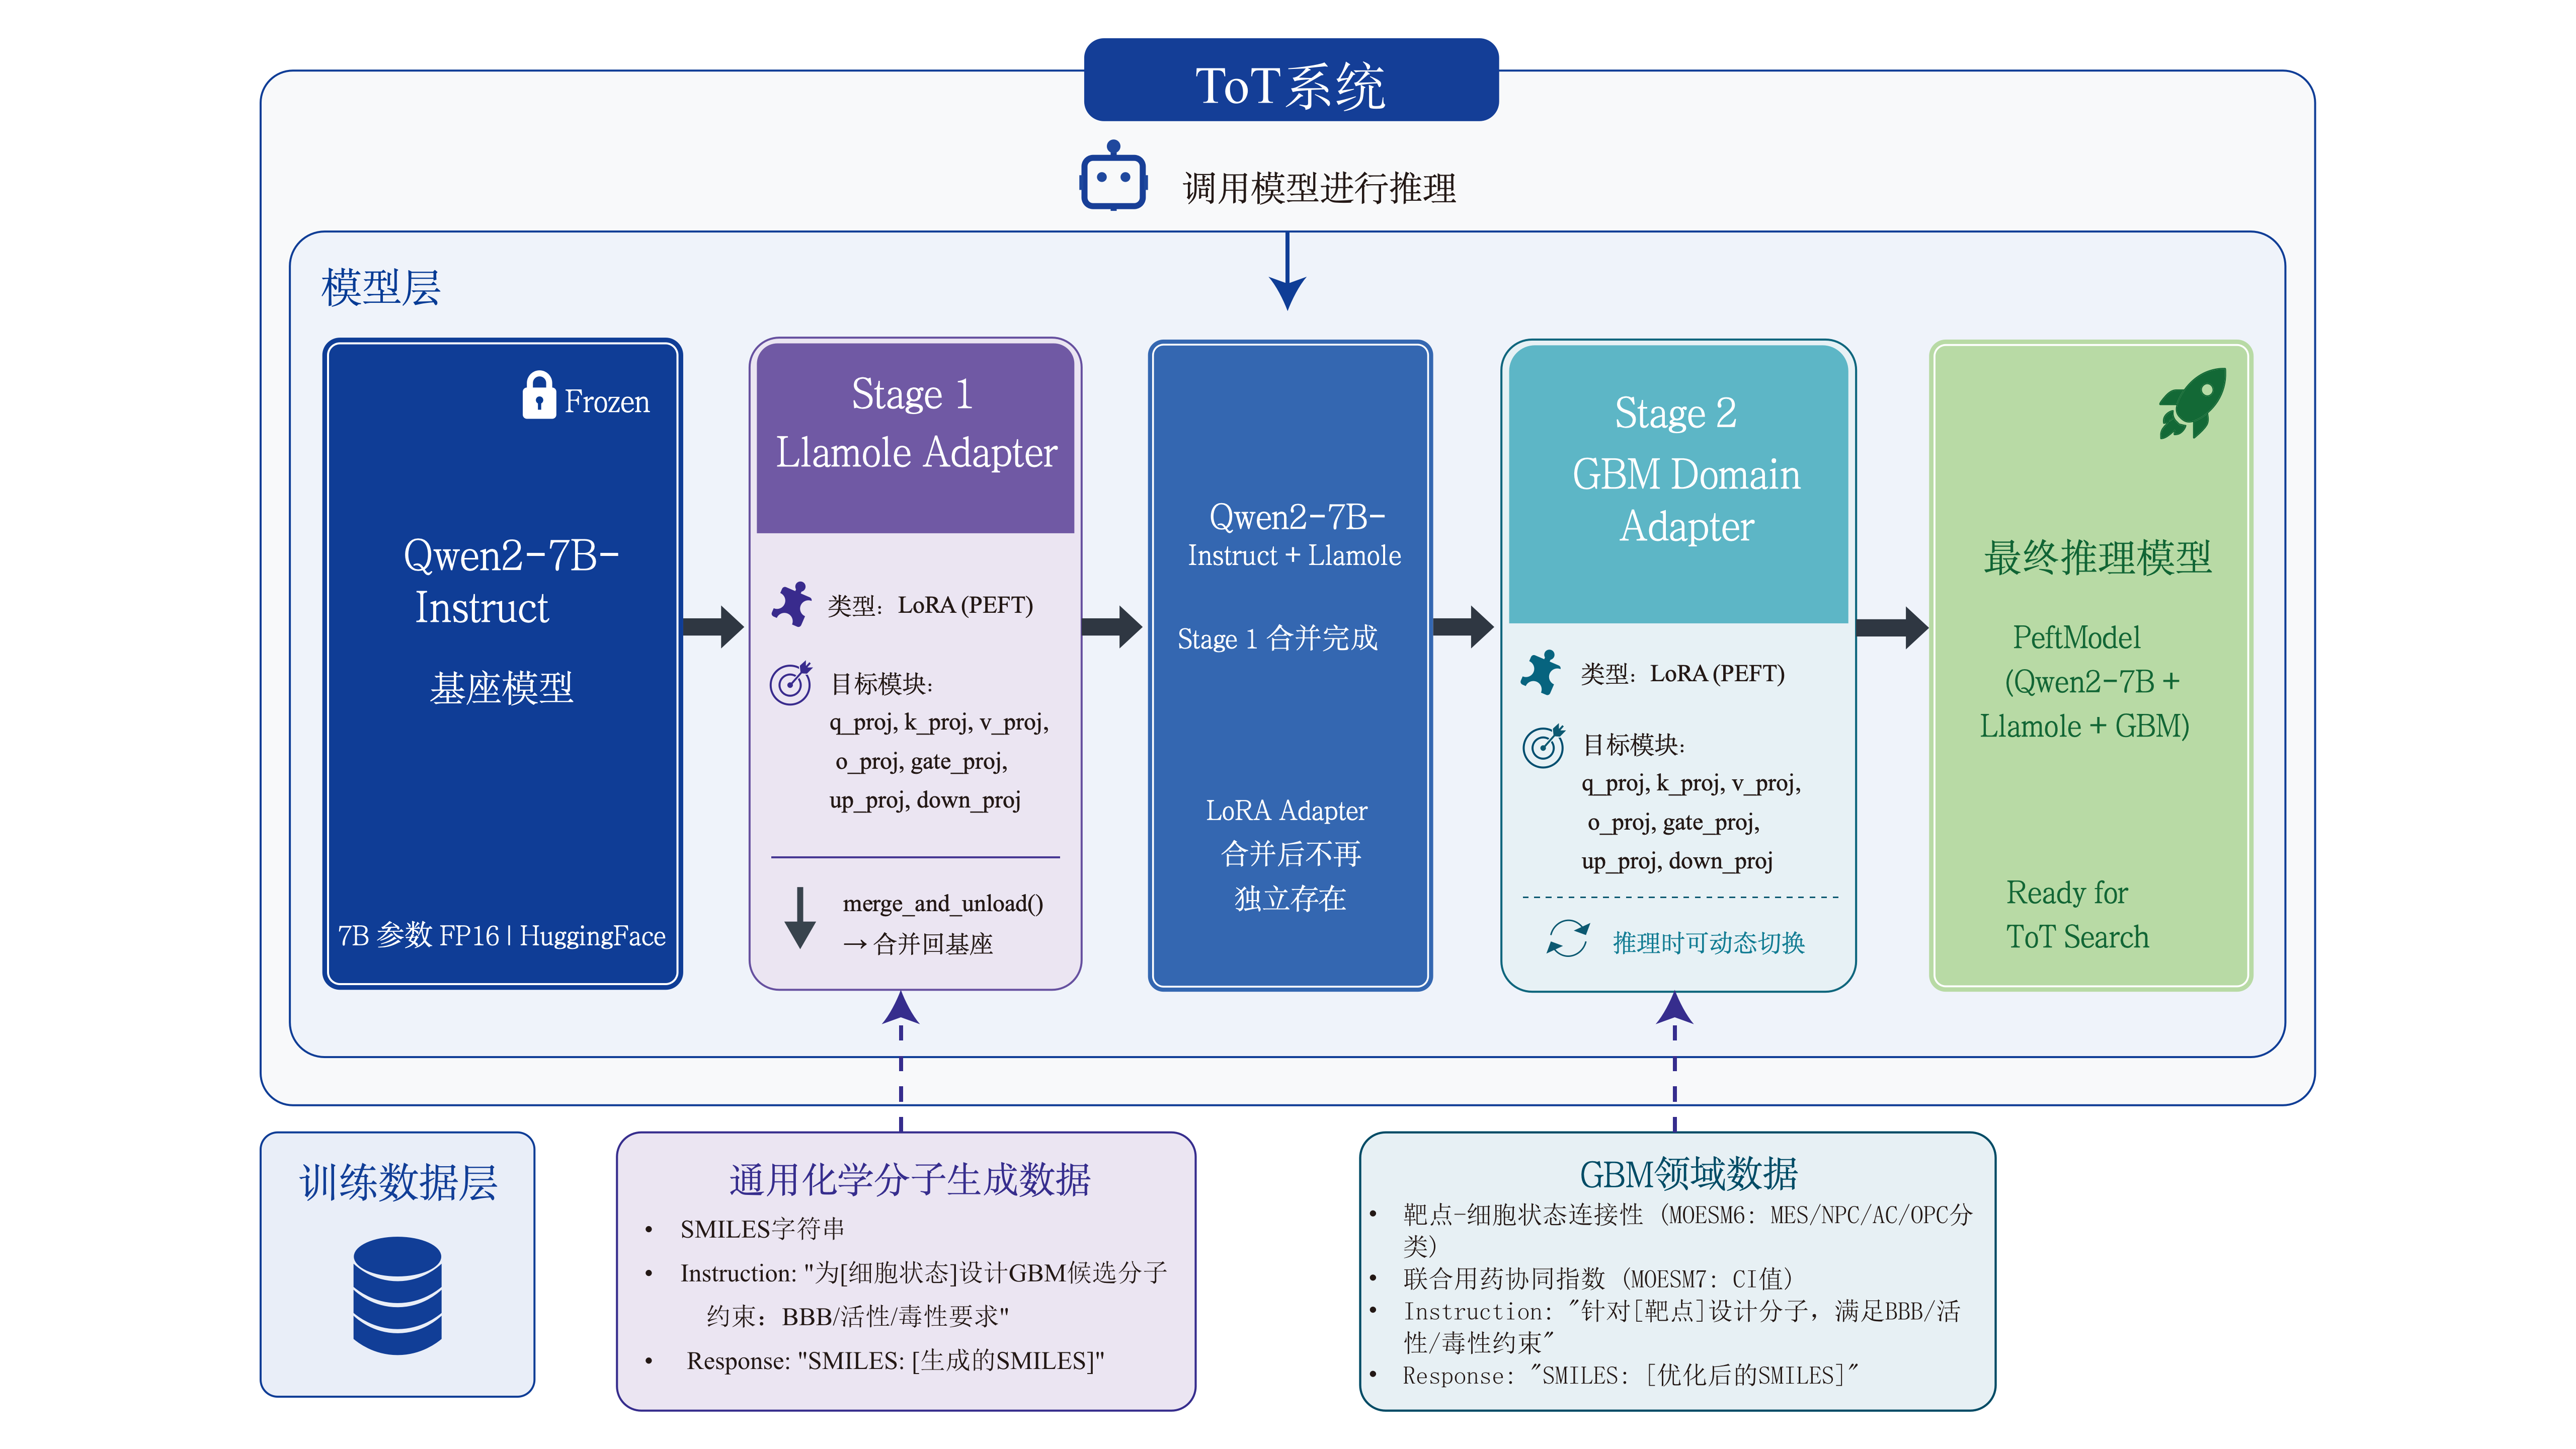
\includegraphics[width=0.9\textwidth]{图片/细节图3.png}
    \caption{GBM领域LoRA适配流程示意图}\label{fig:lora-flow}
\end{figure}

GBM领域LoRA适配可视为作用于基础语言模型参数空间的轻量化领域偏置层。设基础模型参数为$\Theta$，LoRA在目标线性层中引入低秩增量：
$$\Delta W = BA$$
其中，A和B为低秩矩阵，秩参数设置为16。模型实际推理时使用$W+\Delta W$进行计算。该设置使模型在保留原有语言理解能力的同时，引入GBM靶点描述、CNS理化约束和候选分子生成偏好的任务相关信息。本文采用两阶段适配流程：先在通用化学分子生成数据上完成Llamole Adapter适配，再基于GBM领域数据构建GBM Domain Adapter。$r=16$的设置用于在表示能力与训练开销之间取得折中。

LoRA的核心配置参数如表\ref{tab:lora-config}所示：

\begin{table}[htbp]
    \centering
    \caption{LoRA配置参数}\label{tab:lora-config}
    \begin{tabular}{ll}
        \toprule
        \textbf{参数} & \textbf{值} \\
        \midrule
        $r$ (秩) & 16 \\
        lora\_alpha & 32 \\
        lora\_dropout & 0.05 \\
        bias & none \\
        目标模块 & q\_proj, k\_proj, v\_proj, o\_proj, \\
                 & gate\_proj, up\_proj, down\_proj \\
        \bottomrule
    \end{tabular}
\end{table}

选择$r=16$的原因是在表示能力和训练参数之间取得平衡~\cite{hu2022lora}：$r$过小会限制LoRA的表示能力~\cite{hu2022lora}，$r$过大则增加训练开销~\cite{hu2022lora}。$r=16$意味着可训练参数量约为$16 \times (4096 \times 2) \approx 130$K（对于Qwen2-7B的注意力层），远小于全量微调~\cite{hu2022lora}。

\section{CoT-ToT协同生成算法}\label{sec:cot-tot-algorithm}

GBM候选分子生成并不是单一的字符串生成任务，而是同时受到靶点条件、BBB穿透倾向、毒性风险和基础理化性质约束的多阶段生成任务。若直接要求模型一次性输出完整SMILES，模型虽然可以给出形式上可解析的分子字符串，但其中的骨架选择、片段修饰和成药性考虑往往混杂在同一输出中，后续难以判断问题来自结构设计阶段还是来自SMILES表达阶段。因此，本文将CoT推理与ToT搜索结合，用于把候选分子生成过程拆分为更清晰的中间步骤。

本文框架中，CoT主要承担生成过程中的步骤组织作用。模型首先根据靶点背景和CNS药物设计要求，对候选分子的设计方向进行分解，明确骨架选择、局部修饰和最终结构表达之间的先后关系。ToT则用于在每个阶段保留多个候选方向，避免生成过程过早固定在单一结构路径上。两者结合后，模型不再只沿着一条线性推理链生成分子，而是可以在若干候选骨架和片段方案之间进行比较，并将物理评估结果用于后续分支调整。

本文将CoT-ToT生成过程划分为骨架提议、片段组装和SMILES生成三个阶段。骨架提议阶段主要确定候选分子的主体结构和可能的药效团方向，为后续局部修饰提供基础。片段组装阶段在已确定骨架的基础上引入取代基、连接片段或杂环结构，用于扩展候选分子的局部结构空间。SMILES生成阶段则将前两个阶段得到的结构设想转化为可解析的分子字符串，并交由RDKit和物理评估模块进行检查。这样的分阶段设计有助于将分子生成中的结构构思、局部优化和最终表达区分开来，也便于在生成过程中获取反馈信息。

ToT搜索宽度设置为3，主要考虑到候选分支数量与后续物理评估开销之间的平衡。若每一阶段保留过多分支，对接和性质计算的成本会明显增加；若分支数量过少，又容易降低结构探索的多样性。最大深度设置为2，对应骨架、片段和SMILES三个层级。图3.3展示了基于BFS的三阶段搜索流程，模型先生成候选骨架，再围绕保留骨架进行片段组装，最后输出SMILES并进入物理评估。评估结果会被重新写入下一轮Prompt，用于调整后续生成方向，从而形成生成、评估、反馈和再生成的循环。

\begin{figure}[H]
    \centering
    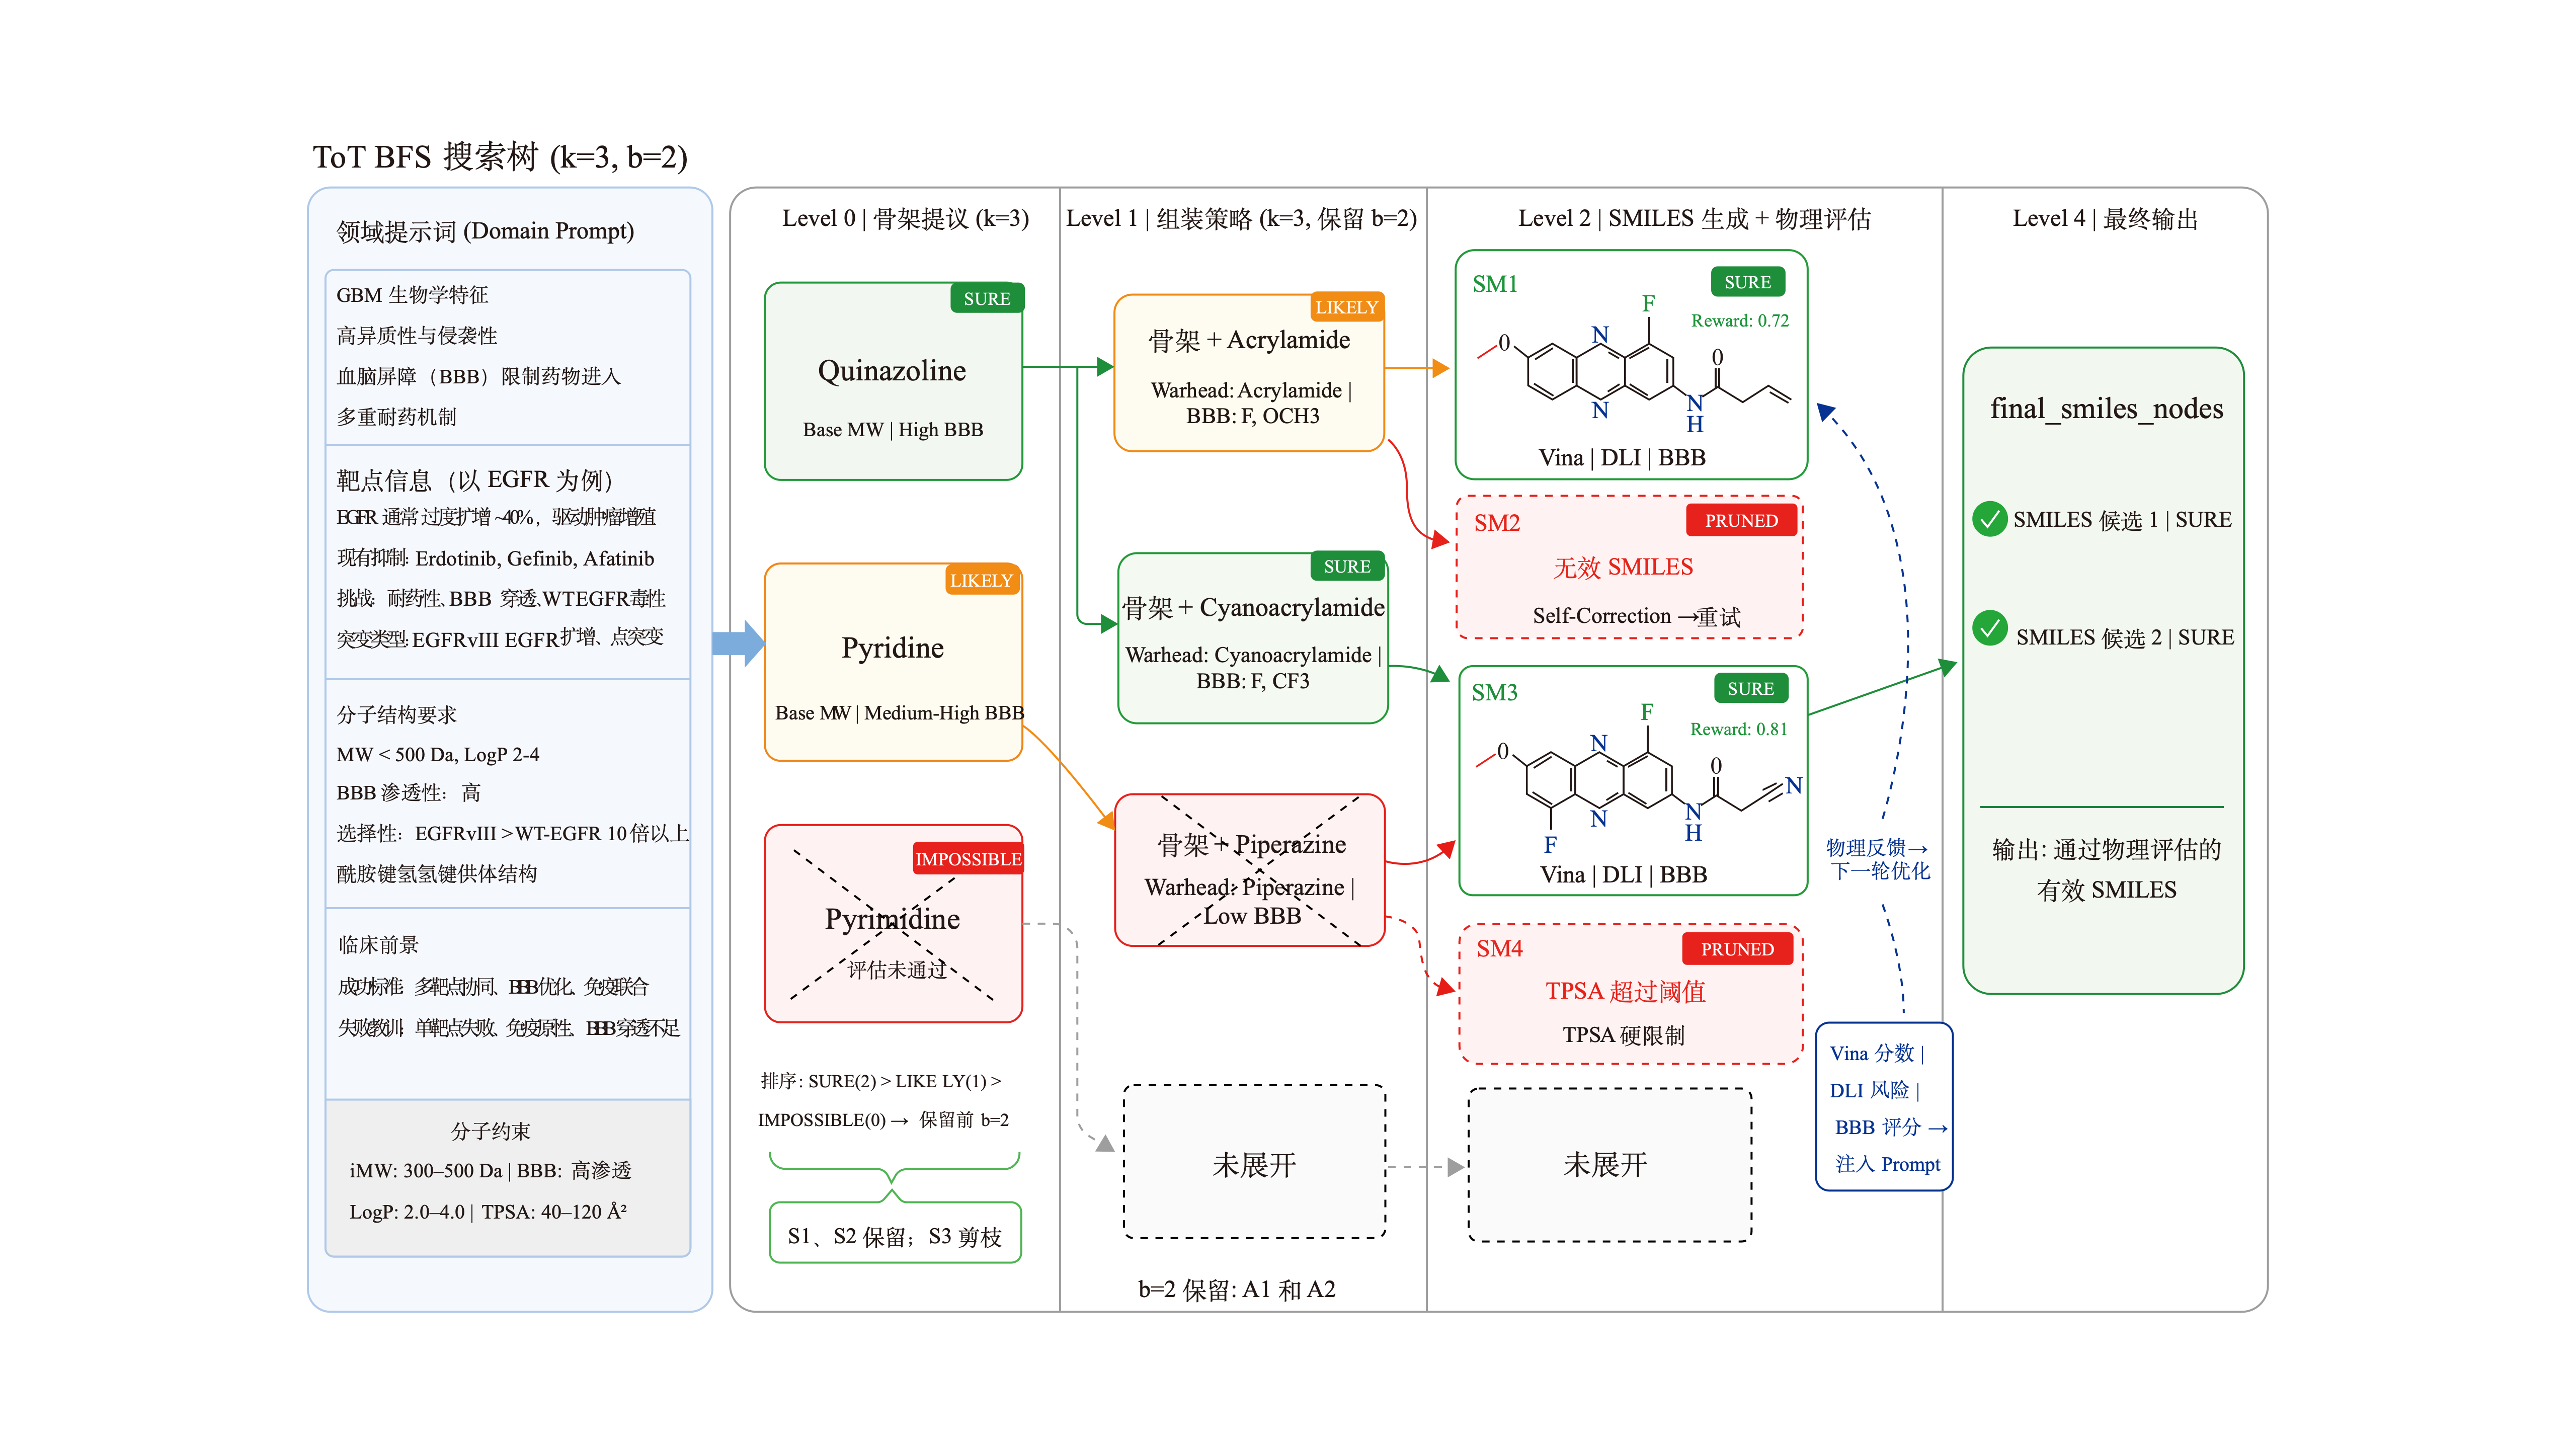
\includegraphics[width=0.9\textwidth]{图片/细节图2.png}
    \caption{基于ToT BFS搜索的三阶段候选分子生成流程示意图}\label{fig:tot-flow}
\end{figure}

该算法的核心伪代码如算法\ref{alg:cot-tot}所示。

\begin{algorithm}
\caption{基于CoT-ToT与物理反馈的GBM候选分子生成算法}
\label{alg:cot-tot}
\textbf{输入}：目标靶点$T$、生成数量上限$N$、知识库$K$、理化约束$C$、搜索宽度$k$、最大深度$d$ \\
\textbf{输出}：候选分子集合$M$及其评分集合$S$

\begin{algorithmic}[1]
\State \textbf{Step 1: 知识检索} \Comment{从知识库中获取靶点相关信息}
\State $K_T \leftarrow \text{QueryTargetKB}(K, T)$
\State $P_{CoT} \leftarrow \text{BuildCoTPrompt}(K_T, C)$ \Comment{构造CoT推理Prompt}

\State \textbf{Step 2: CoT推理} \Comment{使用CoT分解分子设计任务}
\State $R_{CoT} \leftarrow \text{MolecularLLM}(P_{CoT})$ \Comment{获取结构化推理结果}

\State $M \leftarrow \emptyset, S \leftarrow \emptyset$
\State $iter \leftarrow 0$

\While{$|M| < N$ and $iter < MAX\_ITER$}
    \State \textbf{Step 3: 骨架提议（ToT深度0）}
    \State $P_{scaffold} \leftarrow \text{BuildScaffoldPrompt}(R_{CoT}, K_T, C)$
    \State $S_{candidates} \leftarrow \text{MolecularLLM}(P_{scaffold})$ \Comment{生成$k$个候选骨架}
    \State $S_{valid} \leftarrow \text{FilterByBBB}(S_{candidates})$ \Comment{BBB约束预过滤}
    \For{$i \leftarrow 1$ \textbf{to} $|S_{valid}|$}
        \State $scaffold \leftarrow S_{valid}[i]$
        \State \textbf{Step 4: 片段组装（ToT深度1）}
        \State $P_{assembly} \leftarrow \text{BuildAssemblyPrompt}(scaffold, R_{CoT}, C)$
        \State $F_{candidates} \leftarrow \text{MolecularLLM}(P_{assembly})$ \Comment{生成$k$个片段方案}
        \For{$j \leftarrow 1$ \textbf{to} $|F_{candidates}|$}
            \State $fragment \leftarrow F_{candidates}[j]$
            \State \textbf{Step 5: SMILES生成（ToT深度2）}
            \State $P_{smiles} \leftarrow \text{BuildSMILESPrompt}(scaffold, fragment, C)$
            \State $SMILES \leftarrow \text{MolecularLLM}(P_{smiles})$
            \State \textbf{Step 6: SMILES解析与有效性验证}
            \State $mol \leftarrow \text{RDKitParse}(SMILES)$
            \If{$mol \neq \text{None}$ and $\text{IsValidPhysChem}(mol, C)$}
                \State \Comment{Step 7-11: 物理评估管线（生成阶段剪枝反馈）}
                \State $vina \leftarrow \text{VinaDock}(mol, T)$ \Comment{对接分数用于剪枝反馈}
                \State $bbb \leftarrow \text{BBBScore}(mol)$ \Comment{BBB评分用于剪枝反馈}
                \State $dili, herg \leftarrow \text{AlertCheck}(mol)$ \Comment{风险警报用于排除}
                \State $mp \leftarrow \text{MPOReward}(vina, bbb, dili, herg)$ \Comment{中间反馈评分}
                \State $score \leftarrow (vina, bbb, dili, herg, mp)$

                \State \Comment{Step 12: 硬截断与Delta Scoring}
                \If{$\text{HardFilter}(score)$}
                    \State \textbf{continue} \Comment{不合格分子被剪枝}
                \ElsIf{$\text{DeltaCheck}(score, iter) \leq 0.05$}
                    \State \Comment{Delta Scoring豁免：毒性增量不大于0.05时保留}
                \EndIf

                \State $M \leftarrow M \cup \{mol\}$
                \State $S \leftarrow S \cup \{score\}$

                \State \Comment{Step 13: 反馈注入}
                \State $P_{feedback} \leftarrow \text{BuildFeedbackPrompt}(score, R_{CoT})$
                \State $R_{CoT} \leftarrow \text{UpdateCoT}(R_{CoT}, P_{feedback})$
            \EndIf
        \EndFor
    \EndFor
    \State $iter \leftarrow iter + 1$
\EndWhile

\State \textbf{Step 14: Top-$K$排序与输出（基于 TotalScore 的最终排序）}
\State $(M_{sorted}, S_{sorted}) \leftarrow \text{RankByTotalScore}(M, S)$
\State \Return $(M_{sorted}[0:K], S_{sorted}[0:K])$
\end{algorithmic}
\end{algorithm}

该算法实现了"生成—评估—反馈—再生成"的循环：每轮生成后，SMILES生成阶段产生的分子经过物理评估管线打分，反馈结果通过Prompt注入下一轮CoT推理~\cite{Yao2023}，引导模型在下一轮生成时避免低评分分子特征~\cite{Yao2023}。

ToT搜索的三阶段（骨架提议、片段组装和SMILES生成）使得搜索空间逐步聚焦~\cite{Yao2023}：在骨架阶段探索宏观结构（3个分支）~\cite{Yao2023}，在片段阶段探索中观策略（3×3个分支）~\cite{Yao2023}，在SMILES阶段聚焦到具体分子~\cite{Yao2023}。在完成SMILES生成后，系统调用物理评估管线对分子进行打分，评估结果反馈至下一轮CoT推理用于指导改进~\cite{Yao2023}。这种分层搜索策略在探索广度和深度之间取得了平衡~\cite{Yao2023}。

\section{物理评估与闭环反馈}\label{sec:physics-evaluation}

\subsection{物理评估模块的作用}

物理评估模块通过外部工具对生成分子进行多维度量化评价，为候选结构的过滤、剪枝和反馈注入提供依据。该模块接收生成得到的SMILES字符串，并依次计算基础理化描述符、结构风险警报、BBB经验评分、Vina对接分数和MPO Reward，最终形成可用于后续Prompt反馈的评估结果。消融实验结果表明，去除物理评估后DrugCLIP均值下降24.0\%，说明该模块对生成质量具有一定贡献。

为避免生成阶段反馈与最终候选排序在功能上混同，本文将评价指标划分为过程性指标和终局性指标。过程性指标参与生成循环中的过滤、剪枝和反馈注入，终局性指标用于生成结束后的候选分子优先级排序。过程性评价集合可记为：
$$E_g = \{S_{\text{vina}}, S_{\text{BBB}}, A_{\text{DILI}}, A_{\text{hERG}}, R_{\text{MPO}}\}$$
其中，$S_{\text{vina}}$和$S_{\text{BBB}}$分别表示Vina对接分数和BBB经验评分，$A_{\text{DILI}}$与$A_{\text{hERG}}$表示结构风险警报，$R_{\text{MPO}}$表示生成阶段综合反馈得分。终局性指标由TotalScore表示，用于对通过基本过滤的候选分子进行统一排序。

\begin{figure}[htbp]
    \centering
    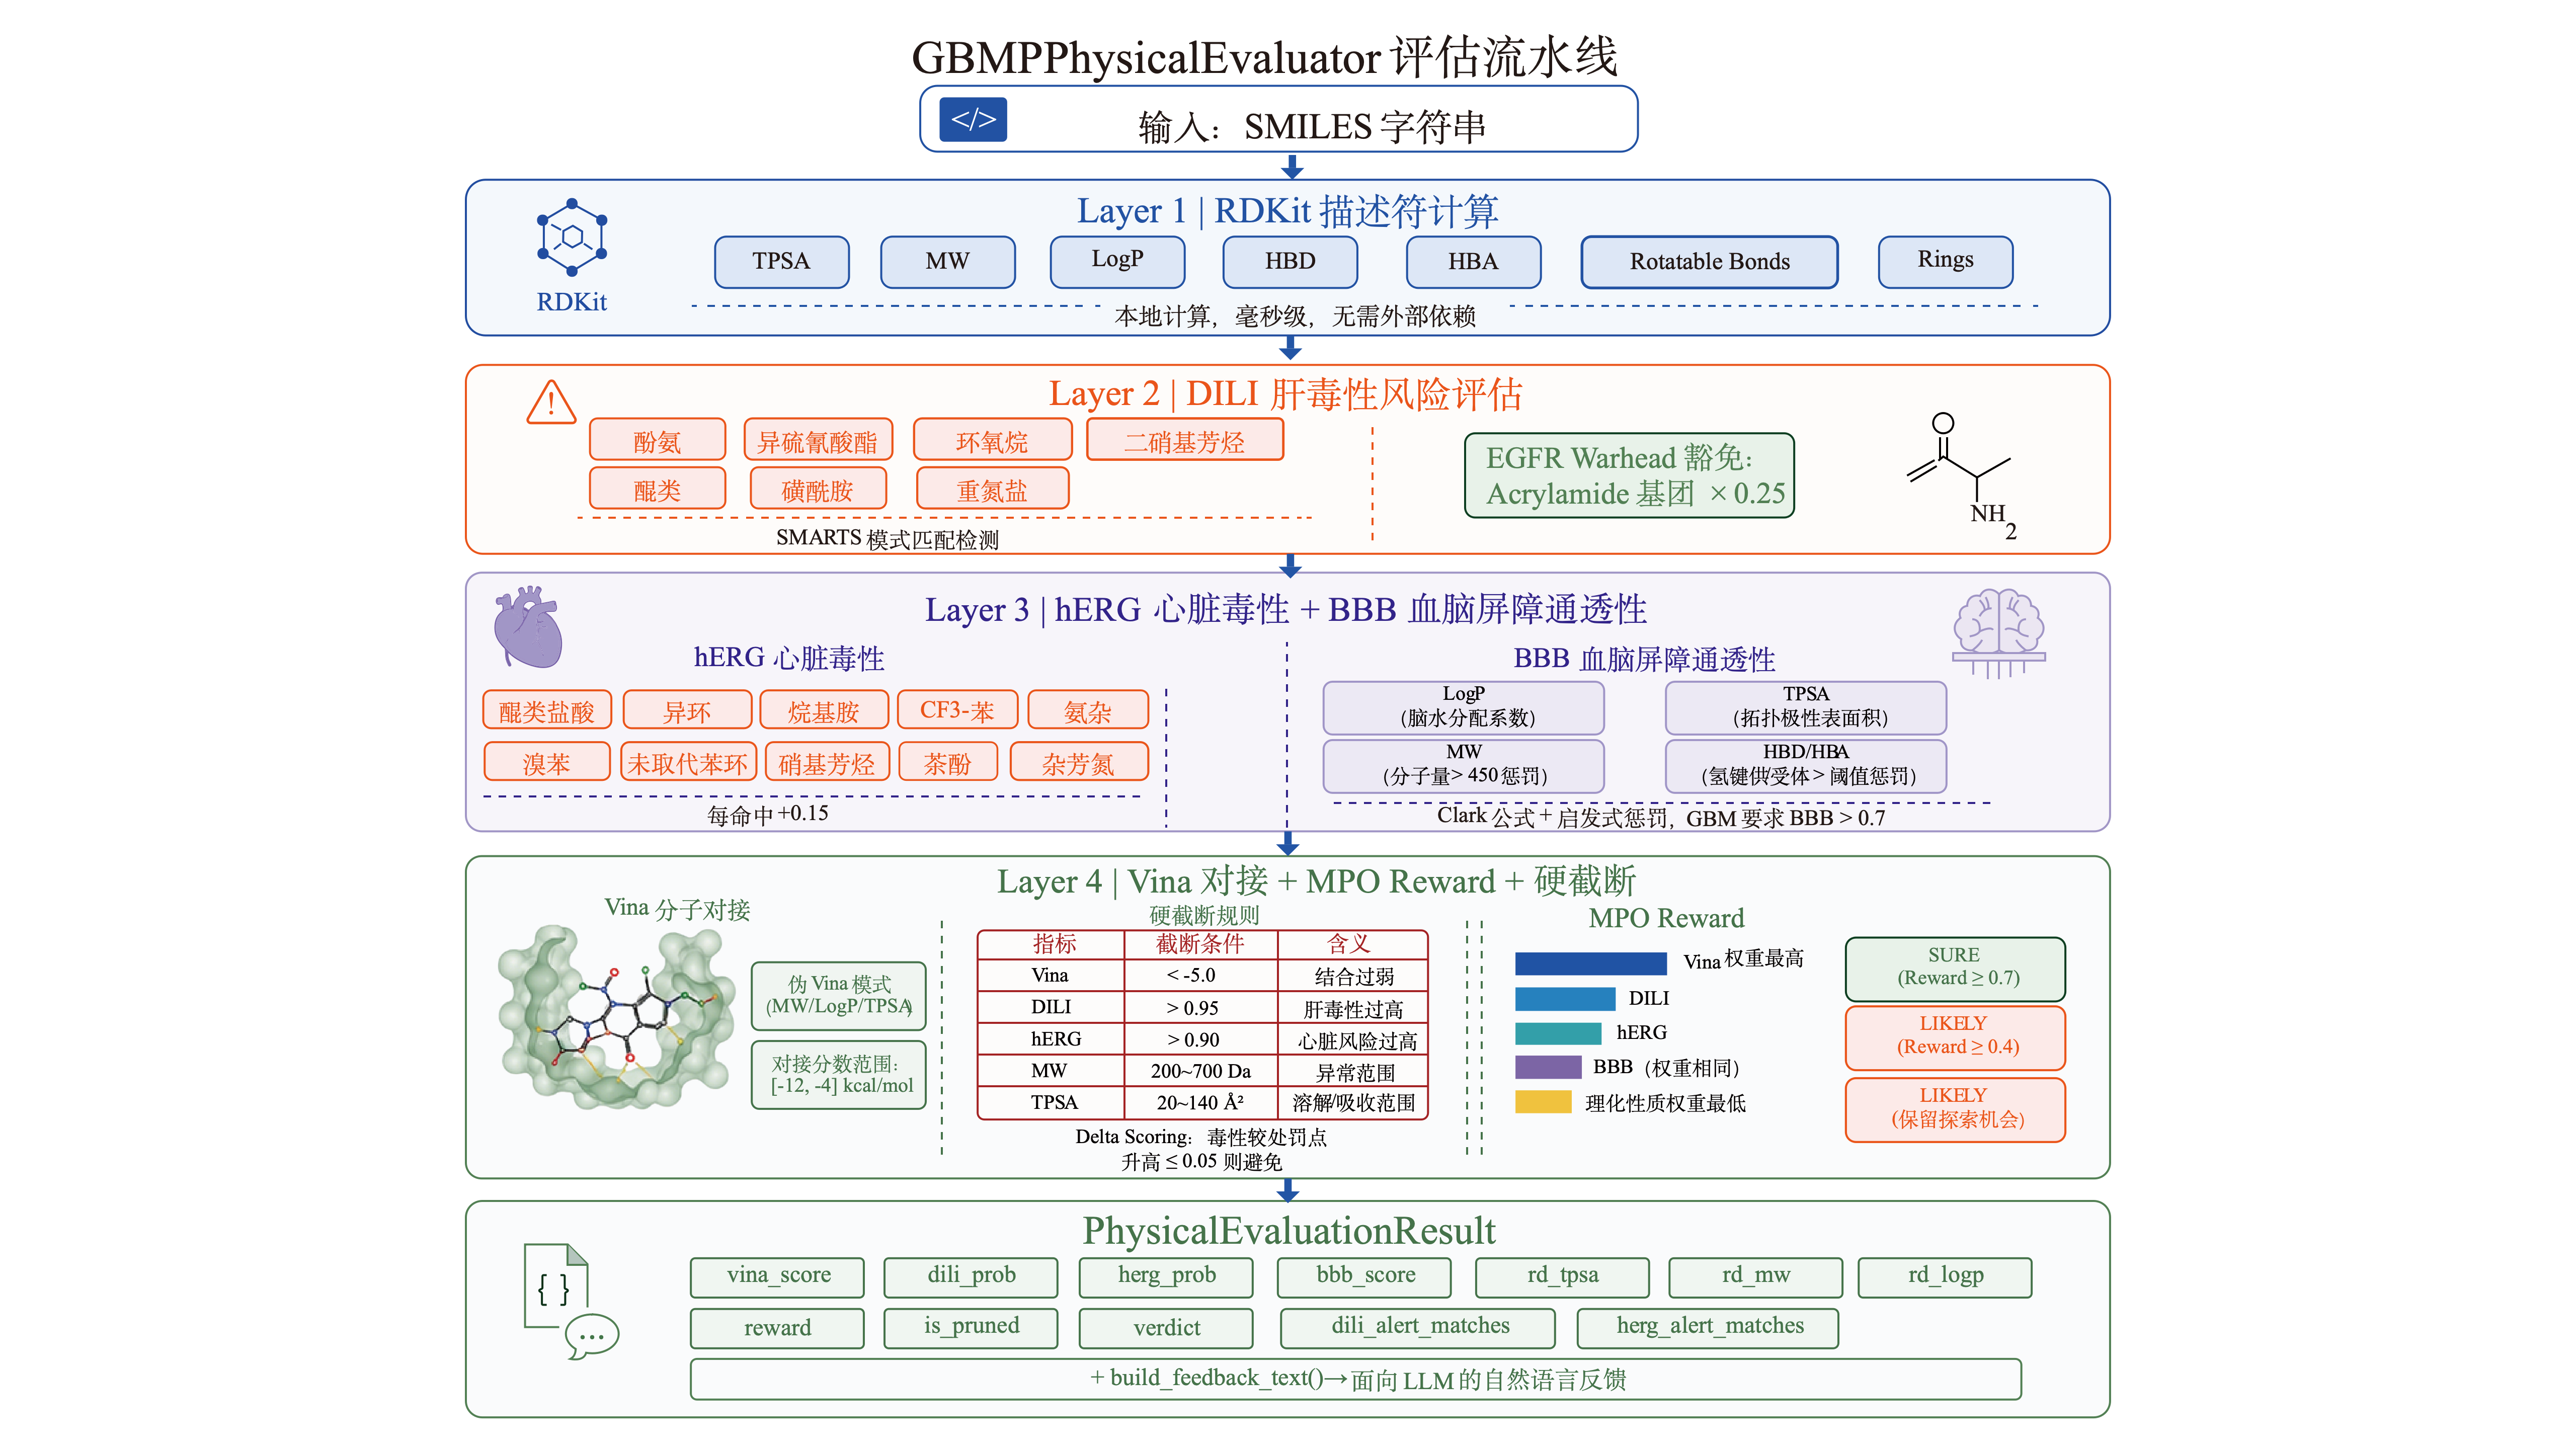
\includegraphics[width=0.9\textwidth]{图片/细节图1.png}
    \caption{GBMPPhysicalEvaluator物理评估流水线示意图}\label{fig:physics-arch}
\end{figure}

\subsection{AutoDock Vina对接}

AutoDock Vina~\cite{Trott2010}用于计算生成分子与靶点蛋白的对接亲和力（kcal/mol）。Vina分数的评估标准为：

\begin{itemize}
    \item Vina < -7.0 kcal/mol：对接分数处于较优区间（强结合参考阈值~\cite{Trott2010}）
    \item -7.0 ≤ Vina < -5.0 kcal/mol：中等结合
    \item Vina ≥ -5.0 kcal/mol：弱结合，触发硬截断剪枝
\end{itemize}

Vina分数在本文中的定位是"生成阶段剪枝反馈"~\cite{Trott2010}，而非"最终排序依据"~\cite{Trott2010}。对接盒子参数配置（如表\ref{tab:docking-box}所示）决定了配体-受体对接的空间范围~\cite{Trott2010}。需要说明的是，Vina对接分数是经验打分~\cite{Trott2010}，\textit{不代表实验结合自由能}，仅用于计算预测结果的相对排序和筛选参考~\cite{Trott2010}。

\begin{table}[htbp]
    \centering
    \caption{对接盒子参数配置}\label{tab:docking-box}
    \begin{tabular}{llcc}
        \toprule
        \textbf{靶点} & \textbf{中心坐标} & \textbf{盒子尺寸（Å）} & \textbf{说明} \\
        \midrule
        EGFR & (-52.5, 15.2, 58.3) & (22.5, 22.5, 22.5) & EGFR激酶域ATP结合位点 \\
        VEGFR2 & (-24.2, 54.6, 52.1) & (22.5, 22.5, 22.5) & VEGFR2疏水口袋 \\
        IDH1 R132H & (12.3, 8.7, -5.2) & (22.5, 22.5, 22.5) & IDH1突变体活性位点 \\
        \bottomrule
    \end{tabular}
\end{table}

\subsection{BBB穿透性预测}

基于LogP与TPSA的经验logBB模型~\cite{Clark2000}用于快速评估CNS药物穿透倾向：

\begin{equation}
\log\text{BB}_{\text{est}} = 0.152 \times \text{LogP} - 0.0148 \times \text{TPSA} + 0.139
\end{equation}

\begin{equation}
\text{BBB\_score} = \frac{\log\text{BB}_{\text{est}} + \text{penalty} + 1.0}{1.5}
\end{equation}

其中penalty项包括：MW > 450时-0.20、HBD > 2时-0.15、HBA > 6时-0.10。

BBB评分在本文中的定位是"生成阶段剪枝反馈"~\cite{Clark2000}，而非"最终排序依据"~\cite{Daina2017}。该方法仅考虑TPSA和LogP~\cite{Clark2000}，\textit{未考虑主动转运和外排泵等机制}，预测结果可能与实际BBB通透性存在偏差~\cite{Pardridge2012}。

CNS药物理化约束参考值为：MW < 450 Da、TPSA < 90 \AA$^2$~\cite{Ertl2000}、LogP 1.0-4.5、HBD ≤ 2、HBA ≤ 7。

\subsection{DILI与hERG风险检测}

基于SMARTS模式匹配的结构警报检测~\cite{Aronov2008}用于快速筛查DILI和hERG风险基团~\cite{Aronov2008}：

\begin{itemize}
    \item \textbf{DILI警报}：酰氯、异硫氰酸酯、环氧烷、醌类等已知肝毒性基团~\cite{Aronov2008}
    \item \textbf{hERG警报}：碱性氮原子（pKa > 8）、萘环、硝基芳香族等已知心脏毒性基团~\cite{Aronov2008}
\end{itemize}

结构警报方法的优势在于计算速度极快（毫秒级），无需外部模型API~\cite{Aronov2008}。

\subsection{MPO Reward综合评分}

MPO Reward使用加权几何平均~\cite{Zhou2019Exp}聚合多维度评分（用于生成阶段中间反馈）：

\begin{equation}
    \text{Reward} = \exp\left(\sum_{i} w_i \cdot \ln(\max(s_i, 10^{-8}))\right)
\end{equation}

MPO Reward的权重配置如表\ref{tab:mpo-weights}所示：

\begin{table}[htbp]
    \centering
    \caption{MPO Reward权重配置}\label{tab:mpo-weights}
    \begin{tabular}{lcc}
        \toprule
        \textbf{指标} & \textbf{权重} & \textbf{归一化方式} \\
        \midrule
        Vina对接分数 & 0.30 & $(-4 - vina) / 8$ \\
        DILI安全性 & 0.20 & $1 - \text{DILI\_prob}$ \\
        hERG安全性 & 0.20 & $1 - \text{hERG\_prob}$ \\
        BBB穿透性 & 0.20 & 直接使用 \\
        理化性质 & 0.10 & $\text{TPSA} \times \text{MW}$几何平均 \\
        \bottomrule
    \end{tabular}
\end{table}

权重设计反映了GBM分子设计的核心需求：Vina对接分数占30\%，BBB穿透性占20\%，DILI和hERG安全性各占20\%，理化性质占10\%。其中，Vina对接分数用于评估生成分子与靶点蛋白的空间匹配程度；BBB穿透性体现了CNS药物设计的核心需求；DILI和hERG安全性用于保证分子的基本安全性；理化性质用于约束分子量和极性表面积等基本属性。

硬截断阈值用于快速过滤明显不合格的分子：Vina > -5.0 kcal/mol、DILI > 0.95、hERG > 0.90、MW < 200或MW > 700、TPSA < 20或TPSA > 140。

Delta Scoring机制允许毒性增量$\le$0.05的分子暂不触发硬剪枝，为探索保留机会~\cite{Zhou2019Exp}。这一设计在保持安全性底线的同时~\cite{Zhou2019Exp}，扩展了分子生成的化学空间~\cite{Zhou2019Exp}。

\section{最终候选分子排序机制}\label{sec:final-ranking}

\subsection{生成阶段剪枝与最终排序的区分}

如上所述，本文明确区分"生成阶段剪枝评价指标"与"最终候选分子筛选排序依据"。这一区分的原因在于：

\begin{itemize}
    \item 生成阶段剪枝（Vina对接、BBB评分、DILI/hERG警报）是为了在生成过程中过滤不合格分子~\cite{Trott2010,Clark2000,Aronov2008}，属于过程控制；
    \item 最终候选排序依据为 TotalScore，用于对通过生成阶段剪枝的候选分子进行综合优先级排序。其中，DrugCLIP 和 SwissADME 结果是 TotalScore 的重要信息来源，但并非唯一排序依据，Vina 对接分数、BBB 穿透性预测、结构风险警报和基础理化性质等指标也共同参与最终评分。
\end{itemize}

两者不能混同：Vina对接分数较高的分子不一定DrugCLIP预测活性高~\cite{Gao2023}；BBB评分合格的分子不一定DrugCLIP预测有活性~\cite{Gao2023}。

\subsection{最终排序依据}

生成阶段的MPO Reward主要服务于剪枝和反馈，不直接决定最终候选分子的优先级。生成结束后，本文使用离线计算得到的TotalScore进行排序。TotalScore综合DrugCLIP预测活性、Vina对接分数、BBB穿透性预测、SA合成可及性、PAINS/Brenk结构警报、P-gp风险和基础理化性质等信息。与生成阶段的局部反馈不同，TotalScore用于对已经通过基本过滤的候选分子进行统一比较，因此更适合作为最终Top候选分子的排序依据。

\section{本章小结}\label{sec:ch3-summary}

本章围绕GBM-PharmaMind框架的结构设计与生成流程进行了系统说明。首先，本文给出了由知识库、生成器和物理评估引擎构成的总体架构；随后，分别介绍了GBM多模态知识库、Prompt生成器、Llamole图—文本生成模块和GBM领域LoRA适配方式；在此基础上，进一步提出CoT-ToT三阶段生成算法，并说明物理评估反馈与最终候选排序之间的功能边界。上述模块共同构成后续实验验证的基础。
